\documentclass[11pt,a4paper]{article}
\usepackage[T1]{fontenc}
\usepackage[utf8]{inputenc}
\usepackage{lmodern}
\usepackage[margin=24mm]{geometry}
\usepackage{amsmath,amssymb,mathtools}
\usepackage{booktabs,longtable,array,tabularx}
\usepackage{xcolor,listings,enumitem}
\usepackage{tikz}
\usetikzlibrary{arrows.meta,positioning}
\usepackage{hyperref}
\usepackage{microtype}
\hypersetup{colorlinks=true,linkcolor=blue!50!black,urlcolor=blue!60!black,citecolor=blue!50!black}
\setlength{\parskip}{5pt}
\setlength{\parindent}{0pt}
\setlength{\emergencystretch}{3em}
\setlist{itemsep=3pt,topsep=4pt}
\lstset{language=Python,basicstyle=\ttfamily\footnotesize,breaklines=true,columns=fullflexible,keepspaces=true,showstringspaces=false,frame=single,rulecolor=\color{black!15},backgroundcolor=\color{black!2},keywordstyle=\color{blue!60!black},commentstyle=\color{green!35!black}}
\newcommand{\clip}{\operatorname{clip}}
\newcommand{\lesson}[1]{\begin{quote}\textbf{Teaching point.} #1\end{quote}}
\title{Understanding an Off-Grid Microgrid with\\Multiple Grid-Forming Battery PCSs\\\large From physical problems to control solutions,\\equations and Python implementation}
\author{Teaching notes for the OffGridMultiGFM project}
\date{October 2026}
\begin{document}
\maketitle
\begin{abstract}
An islanded system must establish its own voltage and frequency while continuously supplying a changing load. Multiple battery power conversion systems increase power and energy capacity, but introduce questions of synchronization, load sharing, unequal battery charge, circulating current and protection. These notes develop the problem and its solutions step by step. Physical reasoning is followed by equations, numerical examples, corresponding Python code and suggested experiments. The reference system has three 5.16 MW PCSs at 690 V and 60 Hz. The implemented simulation is a reduced model with one coherent frequency, per-unit power and control states, and approximate voltage diagnostics. General engineering principles, implemented features and proposed extensions are distinguished throughout.
\end{abstract}
\textbf{Learning objectives.} After working through these notes, the reader should be able to explain why an island requires grid-forming sources; distinguish power adequacy from energy adequacy; derive the signs and units of the control equations; trace each equation into Python; and identify which conclusions the reduced model can and cannot support.

\textbf{Reading plan.} Part I introduces the physical problems and a staged solution. Part II explains the control layers in plain language. Part III works through their mathematics and code. Part IV develops additional analytical checks and guided exercises. Code excerpts refer to the project's actual solver, while explanatory derivations state their additional assumptions.
\tableofcontents
\clearpage
\part{The physical problem and a staged solution}

\section{What is an off-grid battery microgrid?}
A battery stores DC energy. Most facility loads require AC voltage, so a power conversion system (PCS) exchanges energy between the battery and an AC network. In an island, at least one connected source must establish a usable voltage reference. Conceptually, phase-a voltage is
\begin{equation}
v_a(t)=\sqrt{2}V_\phi(t)\sin\theta(t),\qquad \dot\theta(t)=2\pi f(t),
\end{equation}
with the other phases displaced by $120^\circ$. Here $V_\phi$ is phase-to-neutral RMS voltage and $f$ is frequency.

A grid-forming (GFM) inverter maintains an internal voltage reference and adjusts its evolution while exchanging power with the network. A grid-following control primarily synchronizes current injection to an existing voltage reference. That distinction helps explain why an island cannot rely only on controls that require an external reference. The GFM roadmap discusses these control roles and the importance of synchronization, voltage, frequency and protection across time scales~\cite{roadmap}.

The battery supplies energy; the converter and its controller determine how that energy is exchanged. Changing a control gain cannot create additional energy or remove a physical current limit.

\section{The first requirement: satisfy power and energy demand}
\subsection{Instantaneous power adequacy}
In a lossless idealization the desired instantaneous balance is
\begin{equation}
\sum_{i=1}^{N}P_i(t)=P_L(t).
\end{equation}
A real system must also supply losses. During a disturbance, power cannot necessarily adjust instantaneously. Energy in electrical storage elements and source dynamics accommodates the temporary imbalance. The project represents aggregate transient response through a virtual-inertia frequency equation; it does not model the physical energy in every converter capacitor or filter.

If demand exceeds the available discharge power, some combination of additional generation, storage power, load curtailment or shutdown is required. Droop and integral control cannot overcome a sustained infeasible power request.

\subsection{Energy adequacy over an operating period}
The demand over a period is
\begin{equation}
E_L=\int_{t_0}^{t_1}P_L(t)\,dt.
\end{equation}
A system can satisfy an instantaneous MW requirement but still run out of MWh before the required operating time. Conversely, it may contain sufficient energy but lack the converter power to supply a large short peak. Both requirements must be checked independently.
\lesson{Frequency regulation, power sharing and sufficient stored energy are related requirements, but none of them implies the others.}

\section{Why connecting several PCSs is harder than connecting one}
\subsection{A shared AC network requires coordination}
Connecting three voltage sources does not simply add their nameplate ratings. Their phase and frequency trajectories must remain compatible, their power contributions must be feasible, and their voltage references must not cause excessive current exchange.

The conceptual arrangement is shown below. Each battery belongs to its own PCS. A branch includes transformer impedance and the effective impedance produced by control.
\begin{figure}[htbp]
\centering
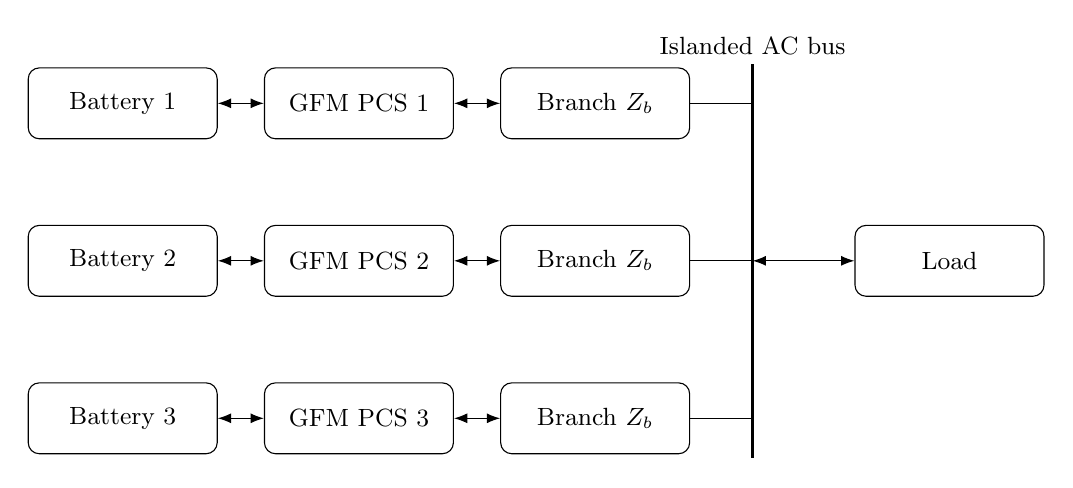
\begin{tikzpicture}[>=Latex,block/.style={draw,rounded corners,minimum height=9mm,minimum width=24mm,align=center},font=\small]
\foreach \i/\yy in {1/2,2/0,3/-2}{
\node[block] (b\i) at (0,\yy) {Battery \i};
\node[block] (p\i) at (3,\yy) {GFM PCS \i};
\node[block] (z\i) at (6,\yy) {Branch $Z_b$};
\draw[<->] (b\i)--(p\i);
\draw[<->] (p\i)--(z\i);
\draw (z\i.east)--(8,\yy);
}
\draw[very thick] (8,-2.5)--(8,2.5);
\node[above] at (8,2.5) {Islanded AC bus};
\node[block] (load) at (10.5,0) {Load};
\draw[<->] (8,0)--(load);
\end{tikzpicture}
\caption{Conceptual three-PCS island. The following tutorial also extends the equations to $N$ identical-rated units. In this drawing $Z_b$ denotes a branch; later equations distinguish the impedance base from actual branch impedance.}
\end{figure}

\subsection{Six problems that must be addressed}
\begin{enumerate}
\item \textbf{Sudden load changes.} Power response takes time. A temporary deficit or excess causes frequency movement.
\item \textbf{Active-power sharing.} Independent converters must contribute cooperatively rather than issuing incompatible commands.
\item \textbf{Frequency restoration.} Primary droop can support demand with a steady frequency offset when references do not fully match the load.
\item \textbf{Unequal battery reserves.} Equal power sharing can deplete the lowest-SoC battery before the others.
\item \textbf{Voltage mismatch.} Magnitude and phase differences can produce current between sources in addition to useful load current.
\item \textbf{Operating limits.} Current, power, DC voltage, temperature and SoC constraints can make the requested operating point infeasible.
\end{enumerate}
Each problem suggests a different feedback objective. A single controller cannot be tuned meaningfully without specifying which error it is intended to correct.

\section{Build a solution step by step}
\begin{description}[style=nextline]
\item[Step 1: establish the voltage/frequency reference.] Use suitable GFM control at the sources. The reduced project assumes coherent operation and represents it with one common frequency; it does not simulate the process of synchronizing independent sources.
\item[Step 2: add fast primary power response.] Use frequency deviation to request more or less power through droop, with finite converter response and limits.
\item[Step 3: restore nominal frequency.] Add secondary integral action to adjust the power correction when a frequency error persists.
\item[Step 4: allocate energy use.] Add EMS feedforward and relative-SoC correction so high-SoC units receive greater discharge duty.
\item[Step 5: coordinate voltage behavior.] Use appropriate voltage control and impedance shaping. The current project illustrates relative voltage compensation through approximate diagnostics.
\item[Step 6: define behavior at constraints.] Saturate commands, prevent integral windup, detect energy boundaries and define a feasible contingency response. The current model stops at the first battery boundary; redispatch after a trip remains an extension.
\end{description}
These layers operate together. A common design intention is to separate fast inner control, primary response and slower supervisory action, but their actual bandwidths must be evaluated. The current equations do not enforce a strict time-scale hierarchy.

\section{Start from a clearly defined model boundary}
The simulation has one common normalized frequency, one common angle-deviation state, and five states per PCS: actual power, delayed EMS reference, secondary correction, voltage compensation and SoC. Thus the state count is $2+5N$, giving 17 states for three units.

This makes the model useful for aggregate frequency and battery-allocation studies. However, it excludes separate unit angles, a solved AC network, switching dynamics, independent reactive loads and physical current-limit behavior. A smooth coherent frequency curve therefore cannot prove synchronization or hardware-level stability of several real PCSs.

The voltage compensation path is a diagnostic approximation and does not feed back into the active-power dynamics. This separation is a property of this implementation, not a general property of physical microgrids.

\section{Conventions to establish before reading any equation}
Internal power is in watts. Positive PCS power discharges a battery; negative power charges it. Positive external load consumes power. SoC is in percentage points: 70 means 70 percent, not 0.70.

For balanced three-phase nominal values,
\begin{equation}
V_\phi=\frac{V_{LL}}{\sqrt{3}},\qquad Z_{base}=\frac{V_{LL}^2}{S_r}.
\end{equation}
Here $S_r$ is the per-unit rating/power base and also the implemented active-power limit. The code does not implement an apparent-power capability circle simply because a rating symbol is used.

The mathematical normalized frequency variable is $x=(f-f_0)/f_0$. In Python that state is named \texttt{speed}. Python also uses the local name \texttt{x} for branch reactance in ohms. These two meanings must be distinguished.

\clearpage
\part{Control layers: purpose, behavior and limitations}


The system must supply an islanded load from several battery PCS units without a utility grid establishing frequency. A load change creates a temporary power imbalance; unequal battery charge calls for unequal power sharing, while small voltage mismatches can drive current between parallel units. The control layers address these different problems together.

\section{Electrical system and control paths}

\begin{lstlisting}[language={}]
Battery 1  <->  GFM PCS 1  <->  transformer / virtual impedance -+
Battery 2  <->  GFM PCS 2  <->  transformer / virtual impedance -+- Islanded AC bus  <->  Load
Battery N  <->  GFM PCS N  <->  transformer / virtual impedance -+

Load + battery SoCs  ->  EMS allocation  ->  communication lag  ->  Pref_i -+
Common frequency  ->  secondary integral correction  ->  Psec_i --------+ ->  power limit  ->  PCS response  ->  Pi
Common frequency  ->  local active-power droop correction -----------+
Sum of Pi - load  ->  aggregate virtual inertia / damping  ->  common frequency
Pi  ->  battery energy accounting  ->  SoC_i  ->  EMS feedback
Voltage mismatch + estimated Q  ->  voltage compensation  ->  voltage / circulating-current diagnostics
\end{lstlisting}

Each battery supplies its own PCS. Positive power discharges a battery; negative power charges it. The AC bus is represented by one common frequency state. The voltage path is a diagnostic approximation alongside the active-power dynamics.

\section{Control layers at a glance}

\begingroup\small
\setlength{\tabcolsep}{3pt}
\begin{longtable}{p{0.16\textwidth}p{0.19\textwidth}p{0.19\textwidth}p{0.22\textwidth}p{0.14\textwidth}}
\toprule
Layer & What it responds to & What it changes & Problem addressed & Where to look \\
\midrule\endhead
PCS response and power limit & Combined active-power command & Each unit's delivered power & Finite converter response and bounded active-power output & Per-unit power \\
Primary GFM response & Generation--load imbalance and frequency deviation & Common frequency dynamics and droop power correction & Arrests frequency movement and supports rapid load sharing & Frequency and total power \\
Secondary frequency control & Persistent frequency error & Integral power correction in each PCS & Drives frequency back toward nominal when feasible & Secondary-control and frequency plots \\
Supervisory EMS & Load demand and relative battery SoC & Per-unit power allocation through a communication lag & Allocates more discharge to higher-SoC batteries & Per-unit power and SoC \\
Voltage coordination & Compensated internal-voltage differences & Per-unit voltage compensation & Reduces modeled internal-voltage mismatch and estimated circulating current & Voltage, compensation and circulating-current plots \\
Protection & PCS rating and battery SoC boundaries & Clips power commands; stops the run at a SoC boundary & Represents active-power capability and prevents continuation past a battery energy boundary & Power and termination message \\
\bottomrule
\end{longtable}
\endgroup

These layers operate concurrently. Their names describe their jobs; this model does not enforce a strict time-scale hierarchy between every controller.

\section{Fast PCS response and primary grid-forming control}

When the load suddenly increases, delivered power cannot change instantly. Total PCS power initially falls short of demand, and the common frequency decreases. The virtual-inertia equation determines how quickly frequency moves; damping opposes the frequency deviation.

The primary P--f droop term raises each PCS power command when frequency is below nominal and lowers it when frequency is above nominal:

\texttt{droop correction\_i = -Sr  *  x / droop\_fraction}, where \texttt{x = (f - f0) / f0}.

The commanded power passes through a first-order PCS response with time constant \texttt{power\_tau\_s} (default 0.05 s). A smaller \texttt{droop\_fraction} produces a stronger power correction for the same frequency error. Increasing \texttt{inertia\_s} reduces the initial rate of frequency change for a given imbalance; it does not add stored energy or converter capacity.

\textbf{What this solves:} the cluster responds to sudden demand before the EMS reference has fully adjusted. Droop alone can leave a frequency offset if it must supply a persistent correction. In this implementation, load feedforward from the EMS also helps remove the power imbalance.

Actual PWM, inner current/voltage loops and separate inverter phase dynamics are not simulated. Their fast active-power response is represented by the first-order power state.

\section{Secondary frequency restoration}

Each PCS integrates the common frequency error:

\texttt{dPsec\_i/dt = Ki  *  (f0 - f)}.

Below nominal frequency, its secondary correction rises; above nominal, the correction falls. This correction is added to the delayed EMS reference and droop term. With sufficient power and energy headroom and suitable tuning, the combined controls drive frequency toward nominal.

Conditional integration blocks further secondary growth when the combined command is already saturated in the same direction. The integral can move back toward the available range when the error reverses.

\textbf{What this solves:} sustained frequency error and integral windup at the modeled active-power limit. The secondary states all receive the same frequency error and use the same gain, so this layer does not balance battery SoC by itself.

\section{Supervisory EMS and battery SoC balancing}

The EMS begins with equal sharing and adds a relative-SoC correction:

\texttt{target\_i = Pload/N + Ksoc  *  (SoC\_i - average SoC)}.

A battery above the average receives a more positive command: it discharges more, or charges less. A battery below the average discharges less, or charges more. Before saturation, the SoC corrections sum to zero, preserving the total requested load allocation. Clipping individual targets can break that equality; the frequency loop then responds to the remaining imbalance within available headroom.

For the default initial SoCs of \textbf{80\%, 60\%, 70\%}, the average is \textbf{70\%}. With \texttt{soc\_gain\_w\_pct = 150000}, the balancing corrections are \textbf{+1.5 MW, -1.5 MW and 0 MW}. At the initial 3 MW load, the ideal EMS targets are therefore \textbf{2.5 MW, -0.5 MW and 1 MW}, before other corrections. PCS 2 can briefly charge from the islanded bus while the other units supply both it and the external load.

These targets pass through \texttt{communication\_tau\_s} (default 0.2 s). This is a first-order lag representing communication/processing response, not a fixed 200 ms transport delay. Initial delivered power and delayed references start at equal load sharing; they then move toward the SoC-aware targets.

\textbf{What this solves:} unequal energy use across the containers. The EMS tends to bring SoCs closer together; it does not restore their average to a fixed charge target. During positive net load, the cluster's average SoC continues to decrease. With equal battery capacities and no saturation, the ideal balancing time constant is \texttt{E/(100 Ksoc)}; with the accelerated default energy it is about 2 s, before accounting for the other dynamics.

\section{Voltage coordination and circulating-current estimates}

Small voltage-reference differences are assigned to the PCS units using a repeatable random mismatch. The model estimates branch current from active power, estimates inductive reactive consumption, and applies a Q-related voltage droop. A voltage-compensation integrator then moves each compensated internal voltage toward the mean of all units.

Transformer and virtual impedances are combined into an effective branch impedance. The circulating-current diagnostic is the largest pairwise compensated internal-voltage difference divided by \texttt{2 |Z|}, representing two equal branches between a pair of units.

\textbf{What this solves in the approximation:} voltage compensation reduces internal-voltage differences, which reduces the estimated circulating current. Compensation equalizes voltages relative to their mean; it does not restore the absolute bus voltage to nominal. Unequal branch currents can leave different estimated terminal voltages after resistive drops.

The simulation does not solve an AC network, reactive-load sharing or phase-angle-driven circulating currents. The estimated reactive power is branch inductive consumption, not an independently controlled load demand. These voltage calculations do not feed back into active-power dynamics, so their plots cannot establish actual multi-inverter voltage stability.

\section{Power and battery protection}

Each PCS command is limited to +/-its active-power rating. The delivered power approaches that bounded command through the PCS response state. The model does not implement an apparent-power circle or semiconductor current limit.

Battery SoC follows the actual power and configured energy capacity. At the first lower or upper SoC boundary (default 2\% / 98\%), the solver stops and reports the boundary. It does not disconnect that unit and continue with the others.

\textbf{What this solves:} the study respects its modeled active-power capability and identifies when battery energy protection becomes relevant. Continued service after a trip requires load shedding, redispatch and topology-switching logic, which are outside this implementation. No controller can supply sustained demand beyond the cluster's power or available energy.

\section{What happens during the default load steps?}

\begin{enumerate}
\item \textbf{At startup:} 3 MW is supplied equally, then the EMS reallocates power according to the 80/60/70\% initial SoCs. Voltage compensation responds to the initial hardware mismatch.
\item \textbf{At 1 s, demand rises from 3 to 6 MW:} delivered power initially lags demand and frequency falls. Droop immediately adds power correction through the PCS response; the delayed EMS allocation and secondary integrals also adjust.
\item \textbf{As generation catches up:} the imbalance decreases and frequency returns toward 60 Hz. The unit power traces can remain unequal because SoC balancing continues.
\item \textbf{At 3 s, demand falls to 4 MW:} temporary excess generation raises frequency. Droop reduces commands, the EMS lowers its allocation, and the secondary correction adjusts.
\item \textbf{At 5.5 s, demand rises to 5.5 MW:} the same response repeats. The simulation continues to 8 s unless a battery protection boundary is reached first.

\end{enumerate}
The controls divide the work: primary control responds to frequency movement, secondary control restores frequency, the EMS allocates energy use, and voltage compensation reduces estimated voltage mismatch. Their gains interact, so enabling all layers does not guarantee good tuning.

\section{How to investigate each layer}

Use \textbf{Compare scenarios} to change one setting at a time with the same load, battery energy and initial SoCs:

\begin{itemize}
\item Set \texttt{secondary\_w\_hz\_s} to zero to isolate its contribution to frequency restoration. The load-following EMS still acts, so frequency may recover even with secondary control disabled.
\item Set \texttt{soc\_gain\_w\_pct} to zero to compare equal allocation against SoC-aware sharing. Equal power from equal-capacity batteries preserves their initial SoC differences.
\item Increase \texttt{communication\_tau\_s} to examine slower EMS response and the resulting demands on the frequency controls.
\item Set \texttt{voltage\_balance\_gain\_s} to zero to compare the estimated effect of voltage compensation. This changes voltage diagnostics, not the active-power/frequency solution.
\item Increase \texttt{energy\_mwh} to a realistic container capacity to study slower SoC evolution. The default is only \textbf{30 MJ = 0.00833 MWh per unit}, deliberately chosen to make balancing visible in an 8 s demonstration.

\end{itemize}
Check both frequency recovery and power/SoC headroom. Small voltage differences or a completed solver run alone are not evidence of hardware-level stability or protection compliance. See \textbf{Model \& equations} for the exact implemented equations and reconstruction assumptions.

\clearpage
\part{From equations to Python: a guided walkthrough}

The equations below are the equations actually implemented in \texttt{src/offgrid\_gfm/model.py}. Each Python block is an excerpt from that file. NumPy computes the same per-unit equation for all PCS units at once: an array of length \texttt{n} holds one value per unit. A dot over a symbol means its time derivative, not a discrete change between plotted samples.

\subsection{Symbols, units and state layout}

\begingroup\small
\setlength{\tabcolsep}{3pt}
\begin{longtable}{p{0.15\textwidth}p{0.4\textwidth}p{0.35\textwidth}}
\toprule
Symbol & Meaning / units & Python name or setting \\
\midrule\endhead
N & Number of equal-rated units & \texttt{n = c.units} \\
Sr & Per-unit rating, W (used as active-power limit and power base) & \texttt{rating = c.rating\_mw * 1e6} \\
f0, f & Nominal and actual frequency, Hz & \texttt{c.frequency\_hz}, output \texttt{frequency\_hz} \\
x & Normalized frequency deviation, dimensionless & \texttt{speed} \\
Delta theta & Angle deviation relative to nominal rotation, rad & \texttt{y[1]} \\
Pi & Actual PCS power, W; positive = discharge & \texttt{p[i]} \\
ri & Delayed EMS reference, W & \texttt{ref[i]} \\
zi & Secondary integral correction, W & \texttt{sec[i]} \\
ci & Voltage compensation, V & \texttt{comp[i]} \\
si & Battery SoC, percentage points (70 means 70\%) & \texttt{s[i]} \\
Ei & Battery energy, J & \texttt{c.energy\_mwh * 3.6e9} \\
\bottomrule
\end{longtable}
\endgroup

The full state vector is

\[
y=[x,\Delta\theta,P_1,\ldots,P_N,r_1,\ldots,r_N,z_1,\ldots,z_N,c_1,\ldots,c_N,s_1,\ldots,s_N]^T.
\]

\begin{lstlisting}
speed = y[0]
p, ref, sec, comp, s = y[2:].reshape(5, n)
\end{lstlisting}

For three units, the indices are \texttt{x: 0}, \texttt{angle: 1}, \texttt{p: 2--4}, \texttt{ref: 5--7}, \texttt{sec: 8--10}, \texttt{comp: 11--13}, \texttt{soc: 14--16}. Reshaping groups the last 15 entries into five rows; it does not create five independent solvers.

\subsection{Common frequency: power imbalance becomes frequency movement}

Define the imbalance on the total cluster power base:

\[
\Delta P_{pu}=\frac{\sum_{i=1}^{N}P_i-P_L}{N S_r},\qquad
x=\frac{f-f_0}{f_0}.
\]

The normalized swing equation and angle equation are

\[
\dot x=\frac{\Delta P_{pu}-D x}{T_j},\qquad
\dot{\Delta\theta}=2\pi f_0x,\qquad f=f_0(1+x).
\]

\begin{lstlisting}
dspeed = ((p.sum()-demand(at))/(n*rating)-c.damping_pu*speed)/c.inertia_s
\end{lstlisting}

\texttt{p.sum()} is total delivered power; \texttt{demand(at)} supplies load in watts at the solver's current time. Their difference is divided by total cluster rating. \texttt{damping\_pu} is dimensionless and \texttt{inertia\_s} is in seconds, so \texttt{dspeed} has units 1/s. The angle derivative appears as \texttt{2*np.pi*c.frequency\_hz*speed} in the returned derivative vector. The final frequency output is computed from \texttt{c.frequency\_hz*(1+states[0])}.

\textbf{Numerical example:} immediately after the 3  ->  6 MW step, suppose delivered power is still 3 MW and x = 0. With three 5.16 MW units and Tj = 10 s:

\[
\dot f=f_0\dot x=60\frac{(3-6)/15.48}{10}\approx-1.163\ \mathrm{Hz/s}.
\]

This is the initial slope, not a predicted sustained frequency ramp: the controls start changing power immediately afterward. The plotted frequency is the integrated outcome of that changing imbalance. The common angle is tracked but is not used in an AC network or inter-unit phase calculation.

\subsection{EMS allocation and communication lag}

The EMS uses the mean SoC and a bounded allocation:

\[
\bar s=\frac{1}{N}\sum_i s_i,\qquad
u_i=\operatorname{clip}\left(\frac{P_L}{N}+K_s(s_i-\bar s),-S_r,S_r\right),
\qquad \dot r_i=\frac{u_i-r_i}{T_{comm}}.
\]

\begin{lstlisting}
target = np.clip(demand(at)/n + c.soc_gain_w_pct*(s-s.mean()), -rating, rating)
\end{lstlisting}

The lag derivative appears in \texttt{rhs} as:

\begin{lstlisting}
(target-ref)/c.communication_tau_s
\end{lstlisting}

\texttt{K\_s = soc\_gain\_w\_pct} has units W per percentage point; \texttt{s-s.mean()} is an array of relative SoCs. \texttt{np.clip} applies the limits independently to each unit. The target is algebraic and can jump with the load; \texttt{ref} is a state and evolves continuously.

For a constant target, the lag has the response

\[
r_i(t)=u_i+[r_i(t_0)-u_i]e^{-(t-t_0)/T_{comm}}.
\]

After one time constant the reference has moved approximately 63\% toward that fixed target. With Tcomm = 0.2 s, response begins immediately rather than waiting 0.2 s. In the complete model, targets also move as SoCs evolve, so this closed-form expression describes a fixed-target example.

\textbf{Code-to-plot connection:} \texttt{ref/1e6} is exported as \texttt{pcsN\_ems\_mw}; it is available in the results CSV. The dashboard's power panel shows actual \texttt{p/1e6}, which also includes droop and secondary effects and therefore need not equal the EMS target or delayed reference.

\subsection{Secondary control and conditional anti-windup}

Before anti-windup is applied,

\[
\dot z_i=K_i(f_0-f)=-K_if_0x.
\]

\begin{lstlisting}
dsec = np.full(n, -c.secondary_w_hz_s*c.frequency_hz*speed)
\end{lstlisting}

\texttt{K\_i = secondary\_w\_hz\_s} has units W/(Hz*s), so integrating \texttt{dsec} produces a power correction in watts. \texttt{np.full} gives every unit the same frequency-error derivative before checking its own saturation condition.

For example, a frequency error of -0.1 Hz with Ki = 8,000,000 W/(Hz*s) gives a secondary ramp of \textbf{+0.8 MW/s per unit}, while that error persists and the unit is not blocked by anti-windup.

Let the unlimited combined command be ai. The implemented rule is

\[
\dot z_i\leftarrow0\quad\text{if}\quad
(a_i\ge S_r\ \text{and}\ \dot z_i>0)\ \text{or}\
(a_i\le-S_r\ \text{and}\ \dot z_i<0).
\]

\begin{lstlisting}
dsec[((command_unlimited >= rating)&(dsec > 0)) |
     ((command_unlimited <= -rating)&(dsec < 0))] = 0
\end{lstlisting}

This freezes integration only when it would push the combined command farther beyond a limit. It does not reset \texttt{sec} to zero or clip the integral state itself. An error of the opposite sign can still move the integral back. \texttt{sec/1e6} produces the secondary-control plot.

\subsection{Primary droop, combined command and delivered power}

With droop fraction R and PCS response time Tf:

\[
a_i=r_i+z_i-\frac{S_r}{R}x,\qquad
b_i=\operatorname{clip}(a_i,-S_r,S_r),\qquad
\dot P_i=\frac{b_i-P_i}{T_f}.
\]

\begin{lstlisting}
command_unlimited = ref+sec-rating/c.droop_fraction*speed
command = np.clip(command_unlimited, -rating, rating)
\end{lstlisting}

The delivered-power derivative is returned as:

\begin{lstlisting}
(command-p)/c.power_tau_s
\end{lstlisting}

The droop fraction is dimensionless: R = 0.01 means a 1\% frequency deviation corresponds to one unit rating of droop correction before saturation. At 60 Hz, a -0.1 Hz deviation gives

\[
-\frac{5.16\ \mathrm{MW}}{0.01}\frac{-0.1}{60}=+0.86\ \mathrm{MW}
\]

per unit. This is added to the delayed EMS reference and the secondary correction. It is a command contribution, not instantaneous delivered power. With Tf = 0.05 s, \texttt{p} follows the bounded total command continuously. The actual power panel displays these \texttt{p} states and their sum; it does not display the unlimited command.

\subsection{Battery energy and the origin of SoC balancing}

For lossless battery accounting,

\[
E_i=E_{i,\mathrm{MWh}}\,3.6\times10^9\ \mathrm{J},\qquad
\dot s_i=-\frac{100P_i}{E_i}.
\]

\begin{lstlisting}
ds = -p/(c.energy_mwh*3.6e9)*100
\end{lstlisting}

Watts are joules per second, making \texttt{ds} percentage points per second. The default 30 MJ battery delivering 1 MW loses \textbf{3.333 percentage points per second}. At -1 MW it gains the same amount, because charging/discharging efficiencies are not modeled.

Why does the EMS equalize SoC? For equal energy E, ideal instantaneous tracking, no saturation and no extra power corrections, define ei = si - mean(s). The equal load-sharing component cancels when subtracting the mean:

\[
\dot e_i=-\frac{100K_s}{E}e_i,\qquad
 e_i(t)=e_i(0)e^{-t/\tau_{soc}},\qquad
\tau_{soc}=\frac{E}{100K_s}.
\]

For E = 30 MJ and Ks = 150,000 W/percentage point, this ideal time constant is 2 s. Actual curves also reflect communication lag, power response, frequency correction and saturation. The SoC plot displays \texttt{s} directly; the cluster mean can decline even while differences shrink.

\subsection{Voltage droop, compensation and diagnostics}

The three-phase rating defines the base impedance and nominal phase RMS voltage:

\[
V_\phi=\frac{V_{LL}}{\sqrt3},\quad Z_b=\frac{V_{LL}^2}{S_r},\quad
R_b=Z_b(R_{tr,pu}+R_{v,pu}),\quad
X_b=Z_b(X_{tr,pu}+X_{v,pu}).
\]

\begin{lstlisting}
vp = c.voltage_ll_v / np.sqrt(3)
zb = c.voltage_ll_v**2 / rating
r, x = zb*(c.transformer_r_pu+c.virtual_r_pu), zb*(c.transformer_x_pu+c.virtual_x_pu)
\end{lstlisting}

Here the Python name \texttt{x} is branch reactance in ohms, whereas the mathematical x above denotes normalized frequency. Inside \texttt{rhs}, normalized frequency is always named \texttt{speed}. The distinction matters when reading the code.

The diagnostic calculations use fixed nominal phase voltage for the current estimate:

\[
I_i=\frac{P_i}{3V_\phi},\quad Q_i=3I_i^2X_b,\quad
n_q=\frac{q_{droop}V_\phi}{S_r},\quad
V_{raw,i}=V_\phi m_i-n_qQ_i.
\]

\begin{lstlisting}
current = p/(3*vp)
q = 3*current**2*x
raw = vp*(mismatch[:, None] if p.ndim == 2 else mismatch) - c.q_droop_fraction*vp/rating*q
\end{lstlisting}

The seeded multiplier \texttt{mismatch} is mi. The shape check supports both a single evaluation (N values) and post-processing all output times (an N  *  samples array). Squaring current makes this inductive-consumption estimate nonnegative even during charging; it is not a signed reactive-load command.

Compensated internal voltage and its balancing law are

\[
U_i=V_{raw,i}+c_i,\quad \bar U=\frac1N\sum_i U_i,\qquad
\dot c_i=-K_v(U_i-\bar U).
\]

\begin{lstlisting}
_, _, raw, _ = electrical(p, comp)
dv = -c.voltage_balance_gain_s*(raw+comp-(raw+comp).mean())
\end{lstlisting}

Kv has units 1/s. A unit 1 V above the mean with Kv = 10/s receives a compensation derivative of -10 V/s. For constant raw voltages, differences decay with time constant 1/Kv; zero gain disables compensation. The derivatives sum to zero, so the controller corrects relative differences without independently restoring the mean voltage.

The displayed diagnostics are

\[
V_{term,i}=U_i-I_iR_b,\qquad
I_{circ,max}=\max_{i,j}\frac{|U_i-U_j|}{2\sqrt{R_b^2+X_b^2}},\qquad
V_{comp,norm}=\sqrt{\sum_i c_i^2}.
\]

\begin{lstlisting}
internal = raw+comp
circ = np.max(np.abs(internal[:, None, :]-internal[None, :, :]), axis=(0, 1))/(2*np.hypot(r, x))
\end{lstlisting}

\texttt{electrical()} returns terminal voltage as \texttt{raw+comp-current*r}. Post-processing exports \texttt{q/1e6}, terminal phase voltage, \texttt{circ}, and \texttt{np.linalg.norm(comp, axis=0)} to their respective panels. A growing compensation norm can accompany a shrinking circulating-current estimate: the compensation effort is increasing to cancel a mismatch. These are algebraic estimates and compensation states, not a solved network voltage or actual circulating-current measurement.

\subsection{SoC event equations and solver termination}

The two event functions measure remaining distance to the closest battery boundary:

\[
g_{low}(y)=\min_i(s_i-s_{min}),\qquad
g_{high}(y)=\min_i(s_{max}-s_i).
\]

\begin{lstlisting}
def lower(at, state):
    return np.min(state[-n:]-c.soc_min_pct)
def upper(at, state):
    return np.min(c.soc_max_pct-state[-n:])
lower.terminal = upper.terminal = True
lower.direction = upper.direction = -1
\end{lstlisting}

\texttt{state[-n:]} selects the last N states, which are the SoCs. Both functions start positive because initial SoCs must lie strictly inside the limits. A downward zero crossing means at least one battery has reached a bound; \texttt{terminal = True} asks the integrator to stop there. This is why the plots can end before the requested load profile ends. It is not implemented by clipping SoC after a completed integration.

\subsection{How Python advances all these equations together}

\texttt{rhs(at, y)} returns the derivatives in exactly the same order as the state vector:

\begin{lstlisting}
return np.r_[dspeed, 2*np.pi*c.frequency_hz*speed, (command-p)/c.power_tau_s,
             (target-ref)/c.communication_tau_s, dsec, dv, ds]
\end{lstlisting}

\texttt{np.r\_} concatenates two scalar derivatives and five arrays of length N. The initial state is assembled in that same order:

\begin{lstlisting}
p0 = np.full(n, load[0]*1e6/n)
y = np.r_[0., 0., p0, p0, np.zeros(2*n), soc]
\end{lstlisting}

Frequency deviation and angle start at zero; actual power and delayed EMS references start at equal load sharing; secondary and voltage-compensation states start at zero. Unequal initial SoCs then cause the EMS target to differ from the initial reference.

Within each load interval the integration call is:

\begin{lstlisting}
sol = solve_ivp(interval_rhs, (t[i], end), y, method='Radau', rtol=1e-6, atol=1e-7,
                dense_output=True, events=(lower, upper))
\end{lstlisting}

Radau is an implicit adaptive integrator suitable for the combination of fast PCS response and slower control/energy states. It evaluates the whole derivative vector at trial states, adjusts internal time steps to its error tolerances, and locates protection events. The tolerances apply to each state in its native numerical units; they are not a statement of physical model accuracy.

The code splits at every input timestamp. In step mode it evaluates the old load just before an interval's right endpoint, then uses the new load on the next interval. States remain continuous across the load change; their derivatives can change abruptly. This avoids smearing a step across a single integration interval.

\texttt{dense\_output=True} supplies interpolated state values for plotting between accepted solver steps. The exported plot samples are therefore different from the solver's internal time steps. The code samples approximately every 10 ms on short input intervals, capped at 200 output points per interval; long intervals can under-resolve transient extrema in the displayed curves.

Finally, the integrated states are reshaped into five N  *  samples arrays, converted from W to MW where appropriate, and passed to the eight-panel report. The dashboard therefore shows the solution of the coupled differential equations, plus the algebraic electrical estimates evaluated along that solution. Use \textbf{Source \& downloads  ->  model.py} to inspect the complete implementation beside this explanation.
\clearpage
\part{Analytical checks, design extensions and exercises}
\section{Derive the steady offset of primary droop}
Assume identical unsaturated units, no secondary correction, stationary references and a constant load. Let $R_\Sigma=\sum_i r_i$. At equilibrium, the combined power commands give
\begin{equation}
\sum_iP_i=R_\Sigma-\frac{NS_r}{R_f}x.
\end{equation}
The stationary swing equation also requires $\sum_iP_i-P_L=NS_rDx$. Combining them yields
\begin{equation}
x_{ss}=\frac{R_\Sigma-P_L}{NS_r(D+1/R_f)}.
\end{equation}
This makes the usual droop offset explicit: a persistent reference deficit is balanced through a nonzero frequency deviation. However, the project's EMS also follows load. If the summed reference eventually equals demand without clipping, the offset can vanish even with secondary control disabled. The result must be interpreted in the context of the full reference path.

\section{A local stability check for frequency restoration}
\subsection{Make the simplifying assumptions explicit}
Neglect EMS dynamics, saturation and differences between units for this calculation. Hold the reference perturbation at zero. Let $p$ and $z$ be the identical per-unit power and secondary perturbations. The common-mode linear dynamics are
\begin{align}
\dot x&=\frac{p/S_r-Dx}{T_j},\\
\dot p&=\frac{z-S_rx/R_f-p}{T_f},\\
\dot z&=-K_if_0x.
\end{align}
For a trial response proportional to $e^{\lambda t}$, eliminate $p$ and $z$ to obtain
\begin{equation}
T_jT_f\lambda^3+(T_j+DT_f)\lambda^2
+(D+1/R_f)\lambda+\frac{K_if_0}{S_r}=0.
\end{equation}
For positive coefficients, the additional cubic Routh--Hurwitz condition is
\begin{equation}
(T_j+DT_f)(D+1/R_f)>T_jT_f\frac{K_if_0}{S_r}.
\end{equation}
The default settings give a left side of $10.05\times101=1015.05$ and a right side of approximately 46.51. This simplified common-mode system satisfies the condition.

\lesson{Integral action can restore frequency only when its gains and the other dynamics produce a stable response. Increasing the integral gain without checking dynamics is not a valid tuning method.}
This calculation is not a stability certificate for the full SoC-coupled, saturated model, and it says nothing about omitted relative-angle or converter-network modes. It is an explanatory analytical check derived from the implemented equations.

\section{Power and energy feasibility in the demonstration}
The total default active-power rating is $3\times5.16=15.48$ MW. The largest external step-profile load, 6 MW, is below this total. Individual feasibility still depends on allocation: a balancing correction can move one unit closer to its limit than the others.

The default per-unit energy is 30 MJ. At initial SoCs 80/60/70 percent and a lower boundary of 2 percent, the aggregate ideal energy above that boundary is
\begin{equation}
E_{available}=30\,[0.78+0.58+0.68]=61.2\ \mathrm{MJ}.
\end{equation}
The specified load profile consumes
\begin{equation}
E_L=3(1)+6(2)+4(2.5)+5.5(2.5)=38.75\ \mathrm{MJ}.
\end{equation}
The aggregate budget is sufficient in this ideal comparison. It does not guarantee that no individual battery reaches a boundary first. Nor should exact transient equality of load energy and integrated PCS power be assumed: the reduced swing equation includes an aggregate damping term and transient imbalance without a separate physical energy-state accounting for all those effects.

\section{From voltage diagnostics to a physical network model}
The simple source-to-source circuit explains why magnitude balancing is only part of the problem. For two voltage phasors behind their branch impedances,
\begin{equation}
\underline I_{12}=\frac{\underline U_1-\underline U_2}{Z_1+Z_2}
\end{equation}
describes the corresponding two-source loop. With equal magnitudes $U$ and small relative angle $\delta$, the numerator magnitude is approximately $U|\delta|$, with $\delta$ in radians. Equal voltage magnitudes therefore do not eliminate phase-driven current exchange.

In a loaded multi-source network, actual branch currents follow the full network equations. A next-stage model would introduce separate converter angle and voltage states, complex or dynamic branch equations, a load model and physical current limits. Such an extension should be checked against higher-fidelity simulation or measurements before making conclusions about synchronization or fault response.

Virtual impedance also deserves careful interpretation. A conceptual control law is
\begin{equation}
\underline V_{cmd,i}=\underline V_{ref,i}-Z_v\underline I_i.
\end{equation}
It shapes the effective output behavior by changing a reference. It is not necessarily a physical resistor dissipating $I^2R_v$ heat. The current project combines transformer and virtual impedances numerically for diagnostic calculations; it does not implement that complete measured-current inner-loop law.

\section{A practical sequence for developing a more complete solution}
\begin{enumerate}
\item \textbf{Specify the service.} Define island load range, allowed frequency/voltage excursions, operating duration, critical loads and required response to a source trip.
\item \textbf{Check ratings and reserves.} Use intended battery energy, power capability, current limits and realistic loss assumptions. Check both aggregate and per-unit feasibility.
\item \textbf{Verify coherent power response.} Use the reduced model to understand signs, allocation and gain interactions. Confirm equilibrium and energy slopes analytically.
\item \textbf{Add network and independent GFM dynamics.} Represent relative angles, voltage states, branch impedances and reactive load. Check the modes the coherent model excludes.
\item \textbf{Represent constraints explicitly.} An illustrative physical capability circle is $P_i^2+Q_i^2\le S_{rated,i}^2$, but priority logic, current saturation and converter behavior must be specified rather than inferred from that circle.
\item \textbf{Define contingency transitions.} On a battery or PCS trip, update the connected topology, recalculate available power, shed load if needed, and restart dynamics with consistent states. The current solver stops instead.
\item \textbf{Add communication realism.} Sampling, packet loss, quantization and stale data can change supervisory performance. Practical secondary-control research investigates these effects~\cite{secondaryhardware}.
\item \textbf{Validate progressively.} Compare with an electromagnetic-transient model and measured responses across the intended operating range. Agreement in a single nominal load step is insufficient.
\end{enumerate}

\section{Default settings as a teaching reference}
\begin{longtable}{p{.32\textwidth}p{.20\textwidth}p{.36\textwidth}}
\toprule Setting & Default & Interpretation\\\midrule\endhead
PCS count and rating & $3\times5.16$ MW & Equal-rated units\\
Nominal voltage/frequency & 690 V L--L; 60 Hz & Balanced nominal base\\
Inertia time; damping & 10 s; 1 & Normalized swing parameters\\
Droop fraction & 0.01 & One percent frequency deviation per unit of droop correction\\
PCS response time & 0.05 s & Actual-power lag\\
EMS response time & 0.2 s & First-order reference lag\\
Frequency integral gain & $8\times10^6$ W/(Hz$\cdot$s) & Per-unit secondary correction\\
SoC allocation gain & $1.5\times10^5$ W/point & Relative-SoC balancing\\
Battery energy & 30 MJ per unit & Accelerated demonstration\\
Voltage mismatch & $\pm1\%$, seed 42 & Repeatable hardware-reference estimate\\
Transformer $R/X$ & 0.005/0.075 pu & Branch contributions\\
Virtual $R/X$ & 0.01/0.05 pu & Effective control impedance\\
Q-droop fraction & 0.02 & Diagnostic voltage law\\
Voltage balance gain & 10 s$^{-1}$ & Relative compensation dynamics\\
SoC limits & 2 and 98 percent & First crossing stops the run\\
\bottomrule
\end{longtable}

\section{Exercises: explain, calculate, then check in the application}
\begin{enumerate}
\item At a positive load step, which changes immediately: the algebraic EMS target, the delayed EMS reference or delivered PCS power? Which derivatives change?
\item At 59.8 Hz, compute the default droop contribution and the default secondary ramp per unit, before constraints.
\item If all equal-capacity batteries supply equal power with the SoC gain disabled, will their initial SoC differences disappear?
\item Multiply battery energy by 100 while retaining power and gains. What happens to the instantaneous SoC slope and ideal balancing time constant?
\item For a 1 V internal-voltage difference, use the default branch impedances to estimate the pairwise circulating current. Does that calculation include an angle mismatch?
\item Why can one battery reach its boundary even though total remaining energy is sufficient for the external load?
\item Does disabling secondary action necessarily produce a permanent frequency error in this project? Explain the role of EMS load feedforward.
\item What conclusion can be drawn from a successful numerical solve? What additional evidence would be required for a physical multi-inverter stability claim?
\end{enumerate}

\subsection*{Suggested answers}
\begin{enumerate}
\item The target changes algebraically. Power and delayed-reference states stay continuous; their derivatives and the frequency derivative change with the new demand and commands.
\item The droop contribution is $+1.72$ MW per unit. The secondary ramp is $+1.6$ MW/s per unit. Both are subject to combined-command saturation and anti-windup.
\item No. Equal power and capacity give identical SoC slopes, preserving their initial differences in the ideal case.
\item The slope magnitude becomes 100 times smaller and the ideal balancing time becomes 100 times longer. Keeping the same gain is therefore a different energy-balancing time-scale choice.
\item $Z_{base}=690^2/(5.16\times10^6)\approx0.09227\ \Omega$. Thus $R_b\approx0.001384\ \Omega$ and $X_b\approx0.01153\ \Omega$, giving $1/[2\sqrt{R_b^2+X_b^2}]\approx43$ A. No independent phase mismatch is included.
\item Energy distribution and feasible transfer matter. Aggregate energy cannot remove a local power, SoC or availability constraint.
\item No. If total delayed EMS reference ultimately matches demand without clipping, frequency can recover without the secondary loop. The droop-only offset derivation must be applied with its reference assumptions.
\item Numerical success means the chosen equations were integrated successfully within the solver's criteria. Physical validity requires appropriate dynamics and parameters, convergence checks and independent validation.
\end{enumerate}

\appendix
\section{Provenance and interpretation of this document}
The project was reconstructed from supplied photographs of a notebook called \texttt{Off\_grid\_3\_PCSs.ipynb}. The local source \texttt{src/offgrid\_gfm/model.py} defines the implementation explained here. Its normalized swing equation, three-phase impedance base, power saturation, anti-windup and event-based SoC stopping are deliberate choices. The pairwise current estimate uses two equal branch impedances. Exact reproduction of a photographed plot is not the objective.

Analytical examples and stability calculations are derivations from the equations and the assumptions stated here. They are not hardware measurements. Background references provide context for general control principles and practical concerns; they do not validate the particular gains or voltage approximations used by the project.

\section{Using this file in Overleaf}
Create a blank Overleaf project, upload \texttt{offgrid\_multi\_gfm\_teaching.tex}, set it as the main document, and select pdfLaTeX. The file is standalone: diagrams use TikZ, code uses \texttt{listings}, and references use an embedded bibliography. No external images, Python execution, bibliography database or shell escape is needed. Recompile if cross-references or the contents page initially show placeholders.

The code excerpts can be checked in the application's Source \& downloads tab. File \texttt{model.py} contains configuration, differential equations and integration; \texttt{report.py} contains plots and exports; \texttt{app.py} contains the interface.

\begin{thebibliography}{9}
\bibitem{roadmap}
National Renewable Energy Laboratory and collaborators,
\emph{Research Roadmap on Grid-Forming Inverters}, NREL/TP-5D00-73476, 2020.
\url{https://www.nrel.gov/docs/fy21osti/73476.pdf}.
General background on GFM control and research needs.
\bibitem{secondaryhardware}
S. Chakraborty, J. Wang, S. Ganguly and B. Kroposki,
\emph{Development of a Practical Secondary Control for Hardware Microgrids},
ECCE poster, NREL/PO-5D00-91676, 2024.
\url{https://research-hub.nlr.gov/en/publications/development-of-a-practical-secondary-control-for-hardware-microgr/}.
Practical context for communication and measurement effects.
\bibitem{project}
\emph{OffGridMultiGFM project source}, \texttt{src/offgrid\_gfm/model.py}, local project snapshot, October 2026.
Primary definition of the implementation explained in these notes.
\end{thebibliography}
\end{document}
